% IEEE-formatted preliminary article (conference)
\documentclass[conference]{IEEEtran}
\usepackage[utf8]{inputenc}
\usepackage[T1]{fontenc}
\usepackage[spanish]{babel}
\addto\captionsspanish{\renewcommand{\tablename}{Tabla}}
\usepackage{csquotes}
\usepackage{url}
\usepackage{graphicx}
\usepackage{microtype}
\usepackage{adjustbox}
\usepackage{rotating}
\usepackage{booktabs}
\usepackage{cite}
\usepackage{hyperref}
\usepackage{tikz}
\usetikzlibrary{positioning, fit, arrows.meta, calc, patterns, decorations.pathreplacing}

\title{Desarrollo de una celda reconfigurable de CGRA}
\author{\IEEEauthorblockN{Duarte Sanchez David, Jimenez Ulate Eddy, Ruiz Rivera Jeffrey, Esquivel Arias Fabian Zúñiga Ramírez Jose Eduardo}
\IEEEauthorblockA{{davidduarte28, e.jimenez.10, yr1ruiz, fabiesqui22, je.zuniga}@estudiantec.cr}
}
\date{}

\begin{document}
\maketitle

% Loosen line breaking to avoid overfull boxes in two-column layout
\sloppy

%\begin{abstract}
%-Este documento es un borrador preliminar en formato IEEE que incluye título, autores, introducción y estado del arte. Aquí debe ir un resumen de 150--250 palabras describiendo objetivos, metodología y resultados esperados.
%\end{abstract}

\section{Introducción}
%La introducción debe motivar el problema, explicar su importancia y definir los objetivos del trabajo. Incluya contexto, preguntas de investigación y contribuciones principales.

 
Las arquitecturas reconfigurables han sido muy exitosas en la industria debido a que la evolución del software ha presentado una rápida evolución, con diversas aplicaciones,
distintas necesidades de usuario y progreso científico, por lo que el hardware no se puede adaptar en la misma velocidad al software \cite{LeiboLiu}. Sistemas de propósito específico
pueden sufrir de obsolescencia rápida y si el precio del desarrollo y producción del hardware es alto, se vuelve inviable económicamente \cite{LeiboLiu}.

Actualmente, arquitecturas como las FPGA (\textit{Field Programmable Gate Arrays}) han sido ampliamente adoptadas en diversas aplicaciones debido a su flexibilidad y capacidad de personalización, tomando fuerza en Computación de alto desempeño (HPC) por sus siglas en inglés. 
Sin embargo, las FPGAs presentan ciertas limitaciones como tiempos de configuración lentos, largos tiempos de compilación y aunque es algo relativo, bajas frecuencias de operación \cite{Podobas}.

 Debido a lo anterior, se ha tomado un interés en HPC en utilizar arquitecturas como los CGRAs (\textit{Coarse-Grained Reconfigurable Arrays}) que ofrecen una solución intermedia entre los FPGAs y los procesadores de propósito general (GPP).
Los CGRAs son arquitecturas de hardware que conceptualmente permiten que el silicio sea maleable y su funcionalidad pueda reconfigurarse de manera dinámica \cite{Podobas}.
Los CGRA tienen la ventaja de ser uno o dos ordenes de magnitud más eficientes que las FPGAs y más de 2 a 3 ordenes de magnitud más eficientes que los GPPs \cite{LeiboLiu}.

El desarrollo de una celda reconfigurable de CGRA es de gran importancia por su relevancia no solo en HPC, si no también en su adopción en aplicaciones de \textit{Machine-learning}, procesamiento de imágenes y visión por computadora, 
comunicaciones y otras áreas \cite{GuoweiZhu}. Por lo tanto el objetivo de este trabajo es el desarrollo de un CGRA heterogéneo, que posea tentativamente celdas de ruteo de datos,
celdas con bancos de memoria distribuida, celdas de procesamiento escalar y celdas de procesamiento vectorial, con la capacidad de ejecutar programas utilizando el set de instrucciones RISC-V, con la capacidad de ejecutar lógica de ocho, 16 y 32 bits.

La importancia de utilizar este set de instrucciones es que este es un estándar abierto, facilitando su adopción debido a que no requiere pagos por licencias. Este es un set de instrucciones basado en la simplicidad,
haciendo que el diseño de hardware sea sencillo y una implementación más directa \cite{riscv}.


\section{Antecedentes y Trabajo Relacionado}
En los últimos años, las CGRA han ganado un protagonismo significativo como aceleradores de hardware debido a su capacidad para ofrecer un equilibrio excepcional entre la flexibilidad del software y el alto rendimiento del hardware de aplicación específica \cite{LeiboLiu,Podobas}. A diferencia de las arquitecturas de grano fino, las CGRAs operan a nivel de palabra o bloque, lo que reduce sustancialmente la sobrecarga de reconfiguración y enrutamiento, haciéndolas particularmente atractivas para aplicaciones eficientes en el borde (edge computing). El desarrollo e investigación de estas arquitecturas ha sido fuertemente impulsado por la adopción del repertorio de instrucciones (ISA) de código abierto RISC-V \cite{riscv}, cuya naturaleza extensible facilita la creación de Sistemas en Chip (SoC) heterogéneos altamente personalizados.

Investigaciones recientes han demostrado las ventajas de integrar estrechamente núcleos RISC-V con arreglos CGRA para superar el cuello de botella tradicional de Von Neumann. Por ejemplo, \cite{granja} exploran la integración de un acelerador CGRA acoplado a un núcleo de alto rendimiento RISC-V CVA6 enfocado en ecosistemas cloud-edge, mientras que \cite{GuoweiZhu} proponen DVHetero, un entorno de trabajo integral para el diseño y la validación de SoCs heterogéneos basados en esta combinación. 

A nivel de implementación práctica, estas arquitecturas se materializan en esfuerzos de código abierto de vanguardia; repositorios como risc-v-cgra (desarrollado por ECASLab) investigan estas integraciones a nivel de sistema, mientras que proyectos como OpenEdgeCGRA (ESL-EPFL) proporcionan plataformas open-hardware completas. En este último, la arquitectura se compone de una malla bidimensional configurable de Elementos de Procesamiento (PEs) o celdas reconfigurables que interactúan en forma de toroide y comparten registros para maximizar la paralelización de instrucciones con una sobrecarga de memoria mínima. Otro proyecto destacable como OpenCGRA desarrollado por el PNNL(\textit{Pacific Northwest National Laboratory}) el cual generar procesadores reconfigurables de forma parametrizable, de esta manera, permite diseñar el hardaware por código como el tamaño de la malla, el tipo de celdas, cómo se comunican entre ellas, luego se prueba el funcionamiento usando Python y Verilator y finalmente se exporta el diseño a un código de diseño de hardware estándar (HDL) como Verilog.

Para que este tipo de sistemas alcance su máximo potencial, el diseño interno de la celda reconfigurable individual (PE) y las herramientas de compilación asociadas son críticos \cite{satyajit}. Destacan la necesidad de un mapeo consciente del contexto de memoria (context-memory aware mapping) para asegurar una aceleración eficiente desde el punto de vista energético, subrayando que la latencia en el acceso a datos dicta el rendimiento global. En este marco, el diseño y desarrollo de una nueva celda reconfigurable de CGRA se fundamenta en la necesidad de optimizar las interconexiones locales, el acceso determinista a operandos intermedios y la versatilidad de sus operaciones a nivel de ciclo de reloj, retos que continúan siendo áreas de activa exploración en la frontera del diseño de aceleradores heterogéneos.


\section{Análisis de Soluciones Existentes (SOTA)} %Jose
\label{sec:sota}

En la actualidad, existen distintos tipos de CGRAs, donde estos pueden tener un arreglo de PEs homogéneos como es el caso de los CGRA HyCUBE y los DySER \cite{Blocks2022} o pueden ser de tipo hererogéneos como el Plasticine que posee dos tipos de unidad, los PCU y los PMU \cite{plasticine2017}. Otra característica importante a destacar es el tipo de precisión que estos dispositivos pueden soportar, donde muchos de estos están restringidos a solo procesar operaciones de enteros, siendo estos más de propósito general y otros donde si se añade la ventaja de punto flotante para procesos más especializados \cite{exploration_tradeoffs}. 

Los sistemas CGRA ya no se ven como un elemento aislado, estos se presentan en la actualidad como una parte heterogénea de un sistema de arquitectura \cite{dvhetero}.
Además, los CGRA han tomado gran importancia en sistemas HPC \textit{High Performance Computing}, donde estos se ven altamente beneficiados de que los PEs sean de tipo heterogéneo, donde se tenga una mezcla de PEs basicos y complejos \cite{exploration_tradeoffs}. Esto es es altamente importante para funciones matemáticas debido a que las CGRAs tradicionales no lo manejan de manera óptima.



En la tabla \ref{tab:comparativa_sota} se muestra una comparativa de tres tipos de CGRA, la construcción de estos dispositivos puede ser variada, 
generando distintas aplicaciones y \textit{trade-offs} donde estos son usados de acuerdo a la aplicación. 




%El diseño de soluciones óptimas requiere un escrutinio riguroso de las alternativas vigentes en la literatura científica. En esta sección se evalúan las fortalezas y debilidades de los enfoques predominantes en el estado del arte (SOTA), delimitando sus escenarios de viabilidad técnica.
%
%\subsection{Estudio Comparativo de Propuestas Vigentes}
%Las soluciones actuales presentan compromisos fundamentales (\textit{trade-offs}) entre flexibilidad, eficiencia y costo de implementación:
%
%\begin{itemize}
%    \item \textbf{Enfoque Basado en Procesadores de Propósito General (GPP):} Destaca por su alta flexibilidad de programación y madurez en cadenas de desarrollo. No obstante, presenta debilidades críticas en entornos de tiempo real debido al determinismo limitado y un consumo energético ineficiente bajo cargas masivas de datos. Es viable únicamente en escenarios donde las restricciones de potencia y latencia son secundarias.
%    \item \textbf{Enfoque Basado en Aceleradores Dedicados (ASIC):} Ofrece el máximo rendimiento por unidad de área y un consumo energético mínimo. Sin embargo, su rigidez absoluta impide la reconfiguración ante actualizaciones algorítmicas, además de acarrear costos de desarrollo inviables para producciones de bajo volumen.
%    \item \textbf{Enfoque Basado en Lógica Programable (FPGAs / Arquitecturas Reconfigurables):} Representa un punto medio balanceado. Permite la optimización a nivel de bits y paralelismo masivo. Su principal desventaja radica en la alta complejidad de diseño, tiempos de compilación elevados y la gestión compleja de la memoria compartida.
%\end{itemize}
%
%Para ilustrar de forma concisa estos compromisos, la Tabla~\ref{tab:comparativa_sota} resume los criterios de viabilidad tecnológica encontrados en la literatura.
%
\begin{table}[htbp]
\caption{Matriz comparativa de soluciones en el estado del arte}
\label{tab:comparativa_sota}
\centering
\scriptsize
\setlength{\tabcolsep}{3pt}
\resizebox{\columnwidth}{!}{%
  \begin{tabular}{@{}l p{1.9cm} p{1.9cm} p{1.9cm}@{}}
  \toprule
  \textbf{Solución} & \textbf{Fortalezas} & \textbf{Debilidades} & \textbf{Viabilidad} \\
  \midrule
  Propuesta A \cite{adres2004} & Baja latencia, optimización espacial. & Rigidez de hardware, alto tiempo de diseño. & Dominios fijos estables. \\
  \addlinespace
  Propuesta B \cite{hycube2017} & Alta flexibilidad, reconfiguración ágil. & Alto consumo de recursos, \textit{overhead}. & Entornos dinámicos no críticos. \\
  \addlinespace
  Propuesta C \cite{plasticine2017} & Procesamiento masivo por ciclo (OP/s). & Consumo energético restrictivo. & Infraestructura fija/servidores. \\
  \bottomrule
  \end{tabular}%
}
\end{table}

El diseño de estos sistemas no solo es necesario a nivel de \textit{hardware} ahora, también es relevante tomar en cuenta su contraparte de \textit{software} \cite{plasticine2017}. Casos como el presentado en \cite{dvhetero} toman como prioridad la validación, el mapeo, el enrutamiento como problemas igual de importantes que la parte de \textit{hardware}



%
%\subsection{Lista de Desafíos Observados}
%A partir del análisis sistemático del SOTA, se derivan los siguientes desafíos técnicos abiertos que justifican el desarrollo de una nueva alternativa:
%\begin{enumerate}
%    \item[\textbf{D1.}] \textbf{Rigidez Estructural:} Incapacidad de los aceleradores actuales para adaptarse a variaciones dinámicas en el dominio de los datos sin comprometer severamente el \textit{timing}.
%    \item[\textbf{D2.}] \textbf{Eficiencia de Recursos Embebidos:} Degradación del rendimiento de procesamiento por unidad de área o celda cuando se escalan los tamaños de datos.
%    \item[\textbf{D3.}] \textbf{Determinismo Temporal:} Cuellos de botella en la latencia de interconexión que impiden garantizar restricciones de tiempo real estricto.
%\end{enumerate}
%
% =========================================================
% NUEVA INTEGRACIÓN: PROPUESTA DE SOLUCIÓN DE II NIVEL
% =========================================================
\section{Propuesta de Solución y Arquitectura de Segundo Nivel}

\subsection{Descripción General y Alcance}
Presenta una \textbf{celda reconfigurable heterogénea} para CGRA, superando arquitecturas homogéneas con sub-utilización ante cargas heterogéneas \cite{adres2004, hycube2017}. Introduce \textbf{cuatro tipos de celdas especializadas} en un único \textit{fabric}:
\begin{enumerate}
    \item \textbf{Enrutamiento:} FIFOs para flujo dinámico sin bloqueos.
    \item \textbf{Memoria distribuida:} Bancos SRAM locales (1–4 KB) eliminan cuellos de botella.
    \item \textbf{Procesamiento escalar:} ALU multi-precisión (int8/16/32) + bucles hardware.
    \item \textbf{Procesamiento vectorial:} SIMD float32 (4–8 lanes) para 4–8 elementos simultáneos.
\end{enumerate}

La Tabla~\ref{tab:desafios_soluciones} mapea desafíos del SOTA a soluciones.

\begin{table}[htbp]
\centering
\caption{Desafíos SOTA y soluciones propuestas.}
\label{tab:desafios_soluciones}
\normalsize
\begin{adjustbox}{max width=\columnwidth}
\begin{tabular}{@{}p{0.07\textwidth}p{0.33\textwidth}p{0.55\textwidth}@{}}
	\textbf{ID} & \textbf{Desafío} & \textbf{Solución} \\
\midrule
C1 & PEs homogéneos $\to$ sub-utilización & 4 celdas especializadas (enrut., mem., esc., vec.) \\
C2 & Overhead routing $>30\%$ área & Celdas routing dedicadas con FIFOs \\
C3 & Memoria centralizada $\to$ cuellos & SRAM distribuido local (1--4 KB) \\
C4 & Latencia config. RISC-V & CSR + DMA; config. parcial por contexto \\
C5 & Multi-precisión simultánea & ALU escalar int8/16/32; VALU float32 \\
C9 & NoC $\to$ cuello de botella & Malla 2D, enlaces 32 b, FIFOs por crédito \\
\bottomrule
\end{tabular}
\end{adjustbox}
\end{table}

\subsubsection{Novedad Arquitectónica}
Combinación inédita: (a) routing como celda primaria con FIFOs, (b) memoria distribuida por celda, (c) multi-precisión entero-flotante en celdas diferenciadas, (d) acoplamiento nativo RISC-V (RV32IMAF) via CSR + DMA. Ninguna arquitectura revisada (ADRES, HyCUBE, Plasticine, etc.) integra simultáneamente estas 4 características.

\subsubsection{Alcance y Entregables}
\begin{itemize}
    \item \textbf{RTL (VHDL):} 4 celdas + router NoC básico.
    \item \textbf{Integración:} Arreglo $2\times2$ con NoC en malla.
    \item \textbf{Verificación:} Testbench exhaustivo + programas aleatorios \cite{verification_cgra}.
    \item \textbf{Síntesis FPGA:} Segun disponibilidad (recursos + $F_{\max}$).
    \item \textbf{Benchmarks:} Multiplicación matrices, FFT, reducción vectores.
\end{itemize}

Métricas en Tabla~\ref{tab:metricas_hls}.

\begin{table}[htbp]
\centering
\caption{Métricas de evaluación (Flujo HLS + FPGA).}
\label{tab:metricas_hls}
\scriptsize
\begin{adjustbox}{max width=\columnwidth}
\begin{tabular}{@{}p{0.35\linewidth}p{0.20\linewidth}p{0.45\linewidth}@{}}
\toprule
\textbf{Métrica} & \textbf{Unidad} & \textbf{Herramienta} \\
\midrule
Recursos FPGA & LUT/FF/DSP/BRAM & Vitis HLS / Vivado 2023.1 \\
$F_{\max}$ & MHz & Vivado Timing \\
Latencia & ciclos & C/RTL Co-simulación (HLS) \\
Throughput & OP/s, GFlop/s & Análisis analítico ($F_{\max}$ + latencia) \\
Potencia & mW & Vivado Power \\
Speedup SW & $\times$ & SystemC vs. RISC-V (C++) \\
\bottomrule
\end{tabular}
\end{adjustbox}
\end{table}

\subsection{Arquitectura de Segundo Nivel: Componentes}
Topología malla $2\times2$ con NoC (control por créditos). Fig.~\ref{fig:diagrama_2nivel_png} muestra el diagrama.

\begin{figure}[htbp]
    \centering
    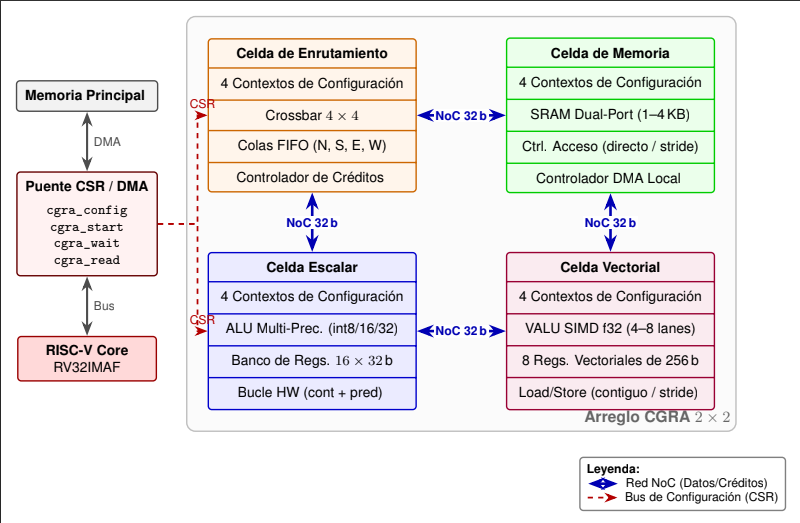
\includegraphics[width=0.9\columnwidth]{images/lvl2_diagram.png}
    \caption{Diagrama de arquitectura de segundo nivel generado con inteligencia artificial.}
    \label{fig:diagrama_2nivel_png}
\end{figure}
\subsubsection{Celda de Enrutamiento}
Primera clase (no multiplexores estáticos): FIFOs 4–8 entradas $\times$ 32 b por puerto; crossbar $4\times4$ (1 ciclo, multicast); control por créditos; 4 contextos (cambio 1 ciclo). Overhead routing $<15\%$ área (vs. $\sim30\%$ en HyCUBE \cite{hycube2017}).

\subsubsection{Celda de Memoria Distribuida}
SRAM dual-port 1–4 KB (BRAM FPGA); controlador (directo/indirecto/stride); interfaz NoC (1–2 ciclos); DMA local (transferencias bloque sin host). Elimina contención centralizada.

\subsubsection{Celda Escalar}
ALU int8/16/32 (4 ops SIMD int8/ciclo); 16 registros $\times$ 32 b; bucles HW (contador + predicación); 4 contextos; interfaz NoC 32 b por crédito.

\subsubsection{Celda Vectorial}
VALU SIMD 4–8 lanes float32 (suma, MAC, reduce); 8 reg. vectoriales (128/256 b); carga/alm. strided; 4 contextos; NoC 128 b (modo ráfaga). Consumirá $\sim3\times$ DSP, entregará $\sim4\times$ throughput float32 \cite{exploration_tradeoffs}.

\subsubsection{Router NoC}
Malla 2D, enlaces 32 b; créditos + FIFO 4 flits; arbitraje round-robin; 1 ciclo/hop; puerto host CSR/DMA (config. celdas, transferencias DMA, lectura resultados).

\subsubsection{Interfaz RISC-V}
CSR dedicado (config. celda, contexto, start/stop); DMA 1 canal; interrupciones/flags; 4 instrucciones custom (cgra\_config/start/wait/read). Reduce latencia config. (desafío C4) \cite{cgra_risc, dvhetero}.

\begin{table*}[htbp]
\centering
\caption{Resumen de componentes.}
\label{tab:resumen_componentes}
\small
\begin{tabular}{@{}p{0.22\textwidth}p{0.30\textwidth}p{0.42\textwidth}@{}}
\toprule
\textbf{Componente} & \textbf{Función} & \textbf{Parámetros clave} \\
\midrule
Enrutamiento & Interconexión + buffering & FIFOs 4–8 $\times$ 32 b; crossbar $4\times4$; 4 contexto \\
Memoria & SRAM distribuido & 1–4 KB dual-port; DMA; 1–2 ciclos \\
Escalar & Entero multi-precisión & int8/16/32; 16 reg.; bucles HW; 4 contexto \\
Vectorial & SIMD float32 & 4–8 lanes; 8 reg.; MAC; 4 contexto \\
Router NoC & Transporte malla & 32 b; créditos; 1 ciclo/hop; round-robin \\
RISC-V & Host-acelerador & CSR + DMA + ISA custom; RV32IMAF \\
\bottomrule
\end{tabular}
\end{table*}

% =========================================================
% NUEVA INTEGRACIÓN: PLAN DE EXPERIMENTO
% =========================================================
\section{Plan de Experimentación y Metodología}%Eddy
\label{sec:experimento}
\subsection{Test y estímulo}

Para probar un diseño electrónico se necesita un testbench, encargado de dirigir un estímulo hacia el diseño y de facilitar el monitoreo de lo que ocurre en el diseño bajo prueba (DUT). Como se ha hecho en otros diseños, y en los distintos frameworks de desarrollo para CGRA, resulta necesario contar con un algoritmo que la arquitectura sea capaz de ejecutar. Para esto se suele partir de los llamados kernels: algoritmos representativos, típicamente codificados en C (por ejemplo, FFT y GEMM), anotados con directivas de compilación sobre los loops, cuya estructura de flujo de datos puede mapearse sobre el arreglo de PEs de una CGRA. Este es, de hecho, el enfoque que sigue Morpher dentro del ecosistema OpenCGRA: a partir del kernel en C genera el grafo de flujo de datos (DFG) y el layout de memoria scratchpad, y produce los vectores de prueba que alimentan la etapa de simulación/emulación, con los que se verifica la correctitud funcional y se obtienen estimaciones de área y potencia \cite{Juneja}. El uso de FFT como kernel de referencia es además consistente con la literatura de CGRA orientada a procesamiento de señales, donde aparece de forma recurrente junto con rutinas como IDCT, FIR e IIR \cite{Podobas}.

Vale la pena notar que incluso en frameworks consolidados como OpenCGRA, sus propios autores señalan que el simulador depende de testbenches escritos manualmente por el usuario y no automatiza la generación de datos de prueba ni las verificaciones de extremo a extremo \cite{Juneja}. Esto refuerza la pertinencia de plantear, desde un inicio, un flujo de pruebas estructurado y progresivo como el que se propone a continuación.

Si bien un objetivo valioso es lograr ejecutar un algoritmo como FFT o GEMM compilado de principio a fin ---desde el programa en C hasta el bitstream de configuración y los datos de entrada de la CGRA---, dado el tiempo disponible para el desarrollo del proyecto, el primer objetivo apunta a pruebas algorítmicamente más sencillas. Se proponen los siguientes pasos:

\begin{enumerate}
    \item \textbf{Una sola PE ejecutando $c = a + b$ (constante) o $c = a \times b$.} Esto valida la carga de la palabra de configuración (config word), la lectura de registros/entradas, la operación de la ALU y la escritura del resultado de salida. Es, literalmente, el ``hello world'' de la arquitectura.
    \item \textbf{Cadenas de operaciones, en modo pipeline:} suma acumulada ($y = x_0 + x_1 + x_2 + \dots + x_n$) y potencias por cuadrados sucesivos ($x,\ x^2,\ x^4,\ x^8,\ \dots$).
    \item \textbf{MAC simple ($acc \mathrel{+}= a \times b$):} es el bloque base de casi todo kernel real (FFT, GEMM, convoluciones), por lo que si esta prueba funciona correctamente, se gana confianza para escalar hacia diseños más complejos.
\end{enumerate}

Una vez superadas estas pruebas básicas, se puede avanzar hacia benchmarks típicos de la literatura de CGRA, como MachSuite y PolyBench \cite{PolyBenchC,MachSuite}, que junto con Wavelib y BEEBS conforman el conjunto de suites utilizado por Morpher para evaluar su flujo de compilación \cite{Juneja}. Estas suites proveen bibliotecas de kernels (incluyendo FFT y GEMM) que pueden mapearse sobre la CGRA mediante un flujo de compilación similar al descrito anteriormente.


\subsection{Monitoreo}

Dado que este proyecto se desarrollará en SystemC, se busca aprovechar las funcionalidades propias del lenguaje para implementar la medición de desempeño. Se propone implementar un monitor como un componente \texttt{SC\_MODULE} que observe, de manera no intrusiva, elementos del DUT como señales y contadores internos. Esta separación entre la lógica funcional y la lógica de medición sigue el principio de diseño modular propio de SystemC, en el que el monitor puede añadirse o removerse del testbench sin modificar el módulo bajo análisis.

Se propone que el monitor calcule, como mínimo, las siguientes métricas:

\begin{itemize}
    \item \textbf{Operaciones por segundo (OP/s):} cociente entre el número total de operaciones ejecutadas por el DUT y el tiempo total de ejecución.
    \item \textbf{Latencia promedio:} registrando \texttt{sc\_time\_stamp()} al inicio y al final de cada operación individual, promediando sobre la ventana de muestreo.
    \item \textbf{Tasa de utilización:} proporción de ciclos activos respecto al total de ciclos.
\end{itemize}

Estas métricas se imprimen a consola mediante \texttt{SC\_REPORT\_INFO}.

Además, cuando el diseño alcance una etapa apta para síntesis en FPGA o ASIC, será posible medir métricas de potencia, área y temporización (\textit{timing}) con las herramientas EDA correspondientes. Esto aplica tanto para la AMD Kria KV260 como para la AMD Alveo U55C.


\subsection{Experimentación arquitectónica}

Ligado a la exploración del espacio de diseño, se plantea generar variaciones del diseño arquitectónico de la CGRA, modificando la cantidad y el tipo de PEs (\textit{processing elements}). Por ejemplo, cambios en la distribución de tipos de PE (más bancos de memoria, más ALUs de punto fijo, más ALUs de punto flotante), así como distintas dimensiones $n \times n$ del arreglo, orientadas a optimizar la ejecución de instrucciones vectoriales.

Este tipo de exploración es consistente con la diversidad de arquitecturas CGRA reportada en la literatura, donde el desempeño depende fuertemente de la composición y disposición de los PEs \cite{Podobas}.

\subsection{Herramientas y Entorno de Desarrollo}
Con el fin de asegurar la reproducibilidad estricta de las pruebas de diseño y simulación, se define la infraestructura de herramientas de software con sus respectivas versiones en la Tabla~\ref{tab:herramientas}.

\begin{table}[htbp]
\caption{Herramientas de Desarrollo y Versiones del Entorno}
\label{tab:herramientas}
\centering
\scriptsize
\begin{adjustbox}{max width=\columnwidth}
\begin{tabular}{@{}p{0.38\linewidth}p{0.18\linewidth}p{0.42\linewidth}@{}}
\toprule
\textbf{Herramienta / Software} & \textbf{Versión} & \textbf{Propósito en el Experimento} \\
\midrule
SystemC & 3.0.1 & Modelado y simulación de la arquitectura CGRA. \\
Xilinx Vivado Design Suite & 2025.2 & Síntesis lógica y análisis de \textit{timing}. \\
ModelSim / Questa Advanced & 2025.1 & Simulación funcional RTL ciclo a ciclo. \\
\bottomrule
\end{tabular}
\end{adjustbox}
\end{table}

\section*{Declaración de uso de herramientas de IA}
Para este trabajo se hizo uso de Inteligencia Artificial para la ayuda en la estructura de la introducción y el estado del arte, así como para una revisión gramatical y ortográfica del documento.


\bibliographystyle{IEEEtran}
\bibliography{references}

\end{document}



%https://github.com/ECASLab/risc-v-cgra/tree/main

%https://github.com/esl-epfl/OpenEdgeCGRA/tree/main

%https://github.com/pnnl/OpenCGRA
